\documentclass{article}
\usepackage{times}
\usepackage{fancyhdr}
\usepackage{extramarks}
\usepackage{amsmath}
\usepackage{amsthm}
\usepackage{amsfonts}
\usepackage{algpseudocode}
\usepackage{pdfpages} %insert pdf pages
\usepackage{enumerate}
\usepackage{listings}
\usepackage{graphicx}




%
% Basic Document Settings
%

\topmargin=-0.45in
\evensidemargin=0in
\oddsidemargin=0in
\textwidth=6.5in
\textheight=9.0in
\headsep=0.25in

\linespread{1.1}

\pagestyle{fancy}
\lhead{\hmwkAuthorName}
\chead{\hmwkClass\  }
\rhead{\hmwkTitle}
\lfoot{\lastxmark}
\cfoot{\thepage}

\renewcommand\headrulewidth{0.4pt}
\renewcommand\footrulewidth{0.4pt}

\setlength\parindent{0pt}


%
% Homework Details
%   - Title
%   - Due date
%   - Class
%   - Section/Time
%   - Instructor
%   - Author
%

\newcommand{\hmwkTitle}{Project \ \#2}
\newcommand{\hmwkDueDate}{February 20, 2015}
\newcommand{\hmwkClass}{Cpr E 550}
\newcommand{\hmwkClassInstructor}{Instructor: Professor Guan Yong}
\newcommand{\hmwkAuthorName}{Chenguang He}

%
% Title Page
%

\title{
    \vspace{2in}
    \textmd{\textbf{\hmwkClass:\\\ \hmwkTitle}}\\
    \normalsize\vspace{0.1in}\small{Due\ on\ \hmwkDueDate\ }\\
    \vspace{0.1in}\large{\textit{\hmwkClassInstructor}}
    \vspace{3in}
}

\author{\textbf{\hmwkAuthorName}}
\date{}

\renewcommand{\part}[1]{\textbf{\large Part \Alph{partCounter}}\stepcounter{partCounter}\\}

\renewcommand{\thesection}{\arabic{section}}% Remove section references...
\renewcommand{\thesubsection}{\arabic{subsection}}%... from subsections



\renewcommand{\thesubsection}{\arabic{subsection}}
\makeatletter
\def\@seccntformat#1{\@ifundefined{#1@cntformat}%
   {\csname the#1\endcsname\quad}%       default
   {\csname #1@cntformat\endcsname}}%    enable individual control
\newcommand\section@cntformat{}
\makeatother

\begin{document}
\maketitle
\newpage
\tableofcontents
\newpage
\section{Implementation Idea}
The entire project contains seven kind of threads: main client, main server, chatroom, UDP multiple client server thread and two prints thread. In order to make the message arrive in order, the project implements the acknowledge just like what it is in TCP and all  threads above are in asynchronous, the main data structure behinds this is the Blockedqueue in Java.\\

After client send the request to join a new created chatroom, the server send back the port name of the chatroom and start a new thread to listen in that port and wait for client connection. The client connect the server's port and start to send message, the server returns a welcome message to ensure the connection has been established. When a chatroom has been created, it also start a print thread, wait for all income message and dispatch them to all user in current chatroom, it add the number of message into blocked queue as same to the number of user in chatroom. Since the connection between user and server are waiting for message in the queue, when a new message arrived in queue, they take them one by one in order. The queue is a blocked queue, which means, the message are taken in the order of the lines of waiting threads, in other words, each message dispatch for each client only once. \\

In the client side, when the connection has been established, the threads create a new thread in order to receiving and printing all messages which send by server. When the client receive a message from server, it acks the message immediately before sending any message, this implementation could ensure the messages acked before sending next message.
\clearpage 

\section{Thread Model}
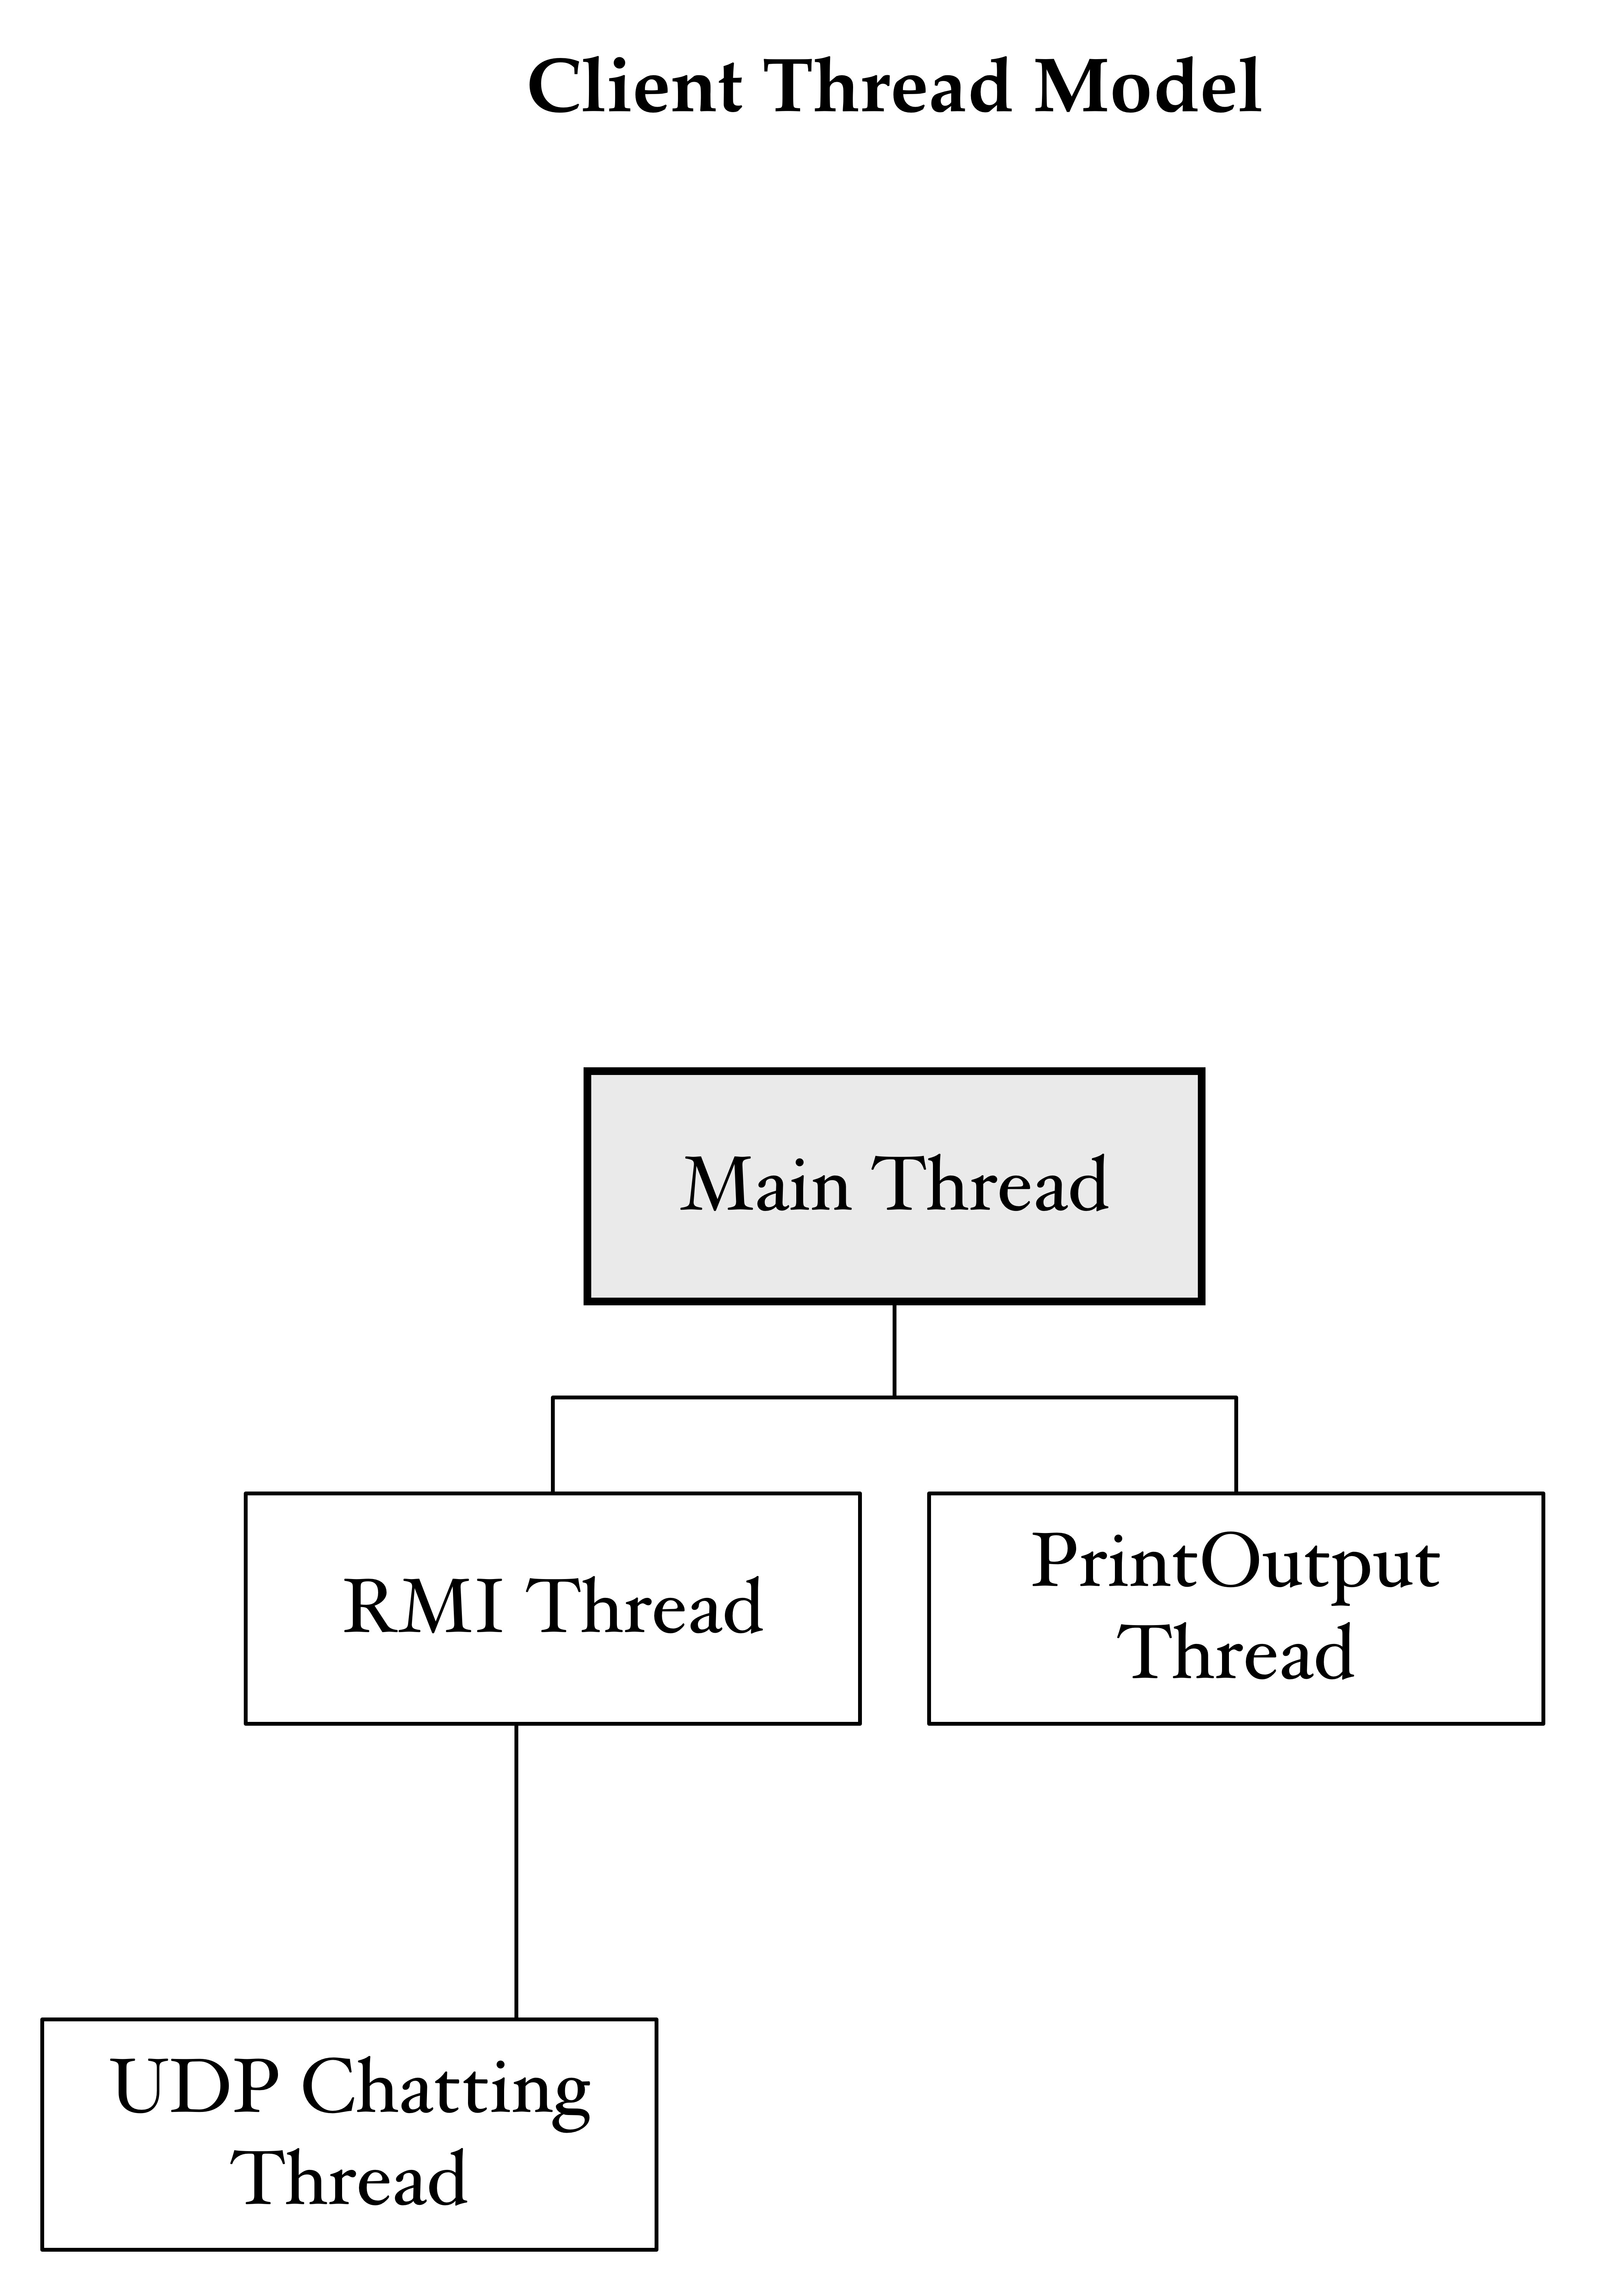
\includegraphics[scale=0.05]{Client}
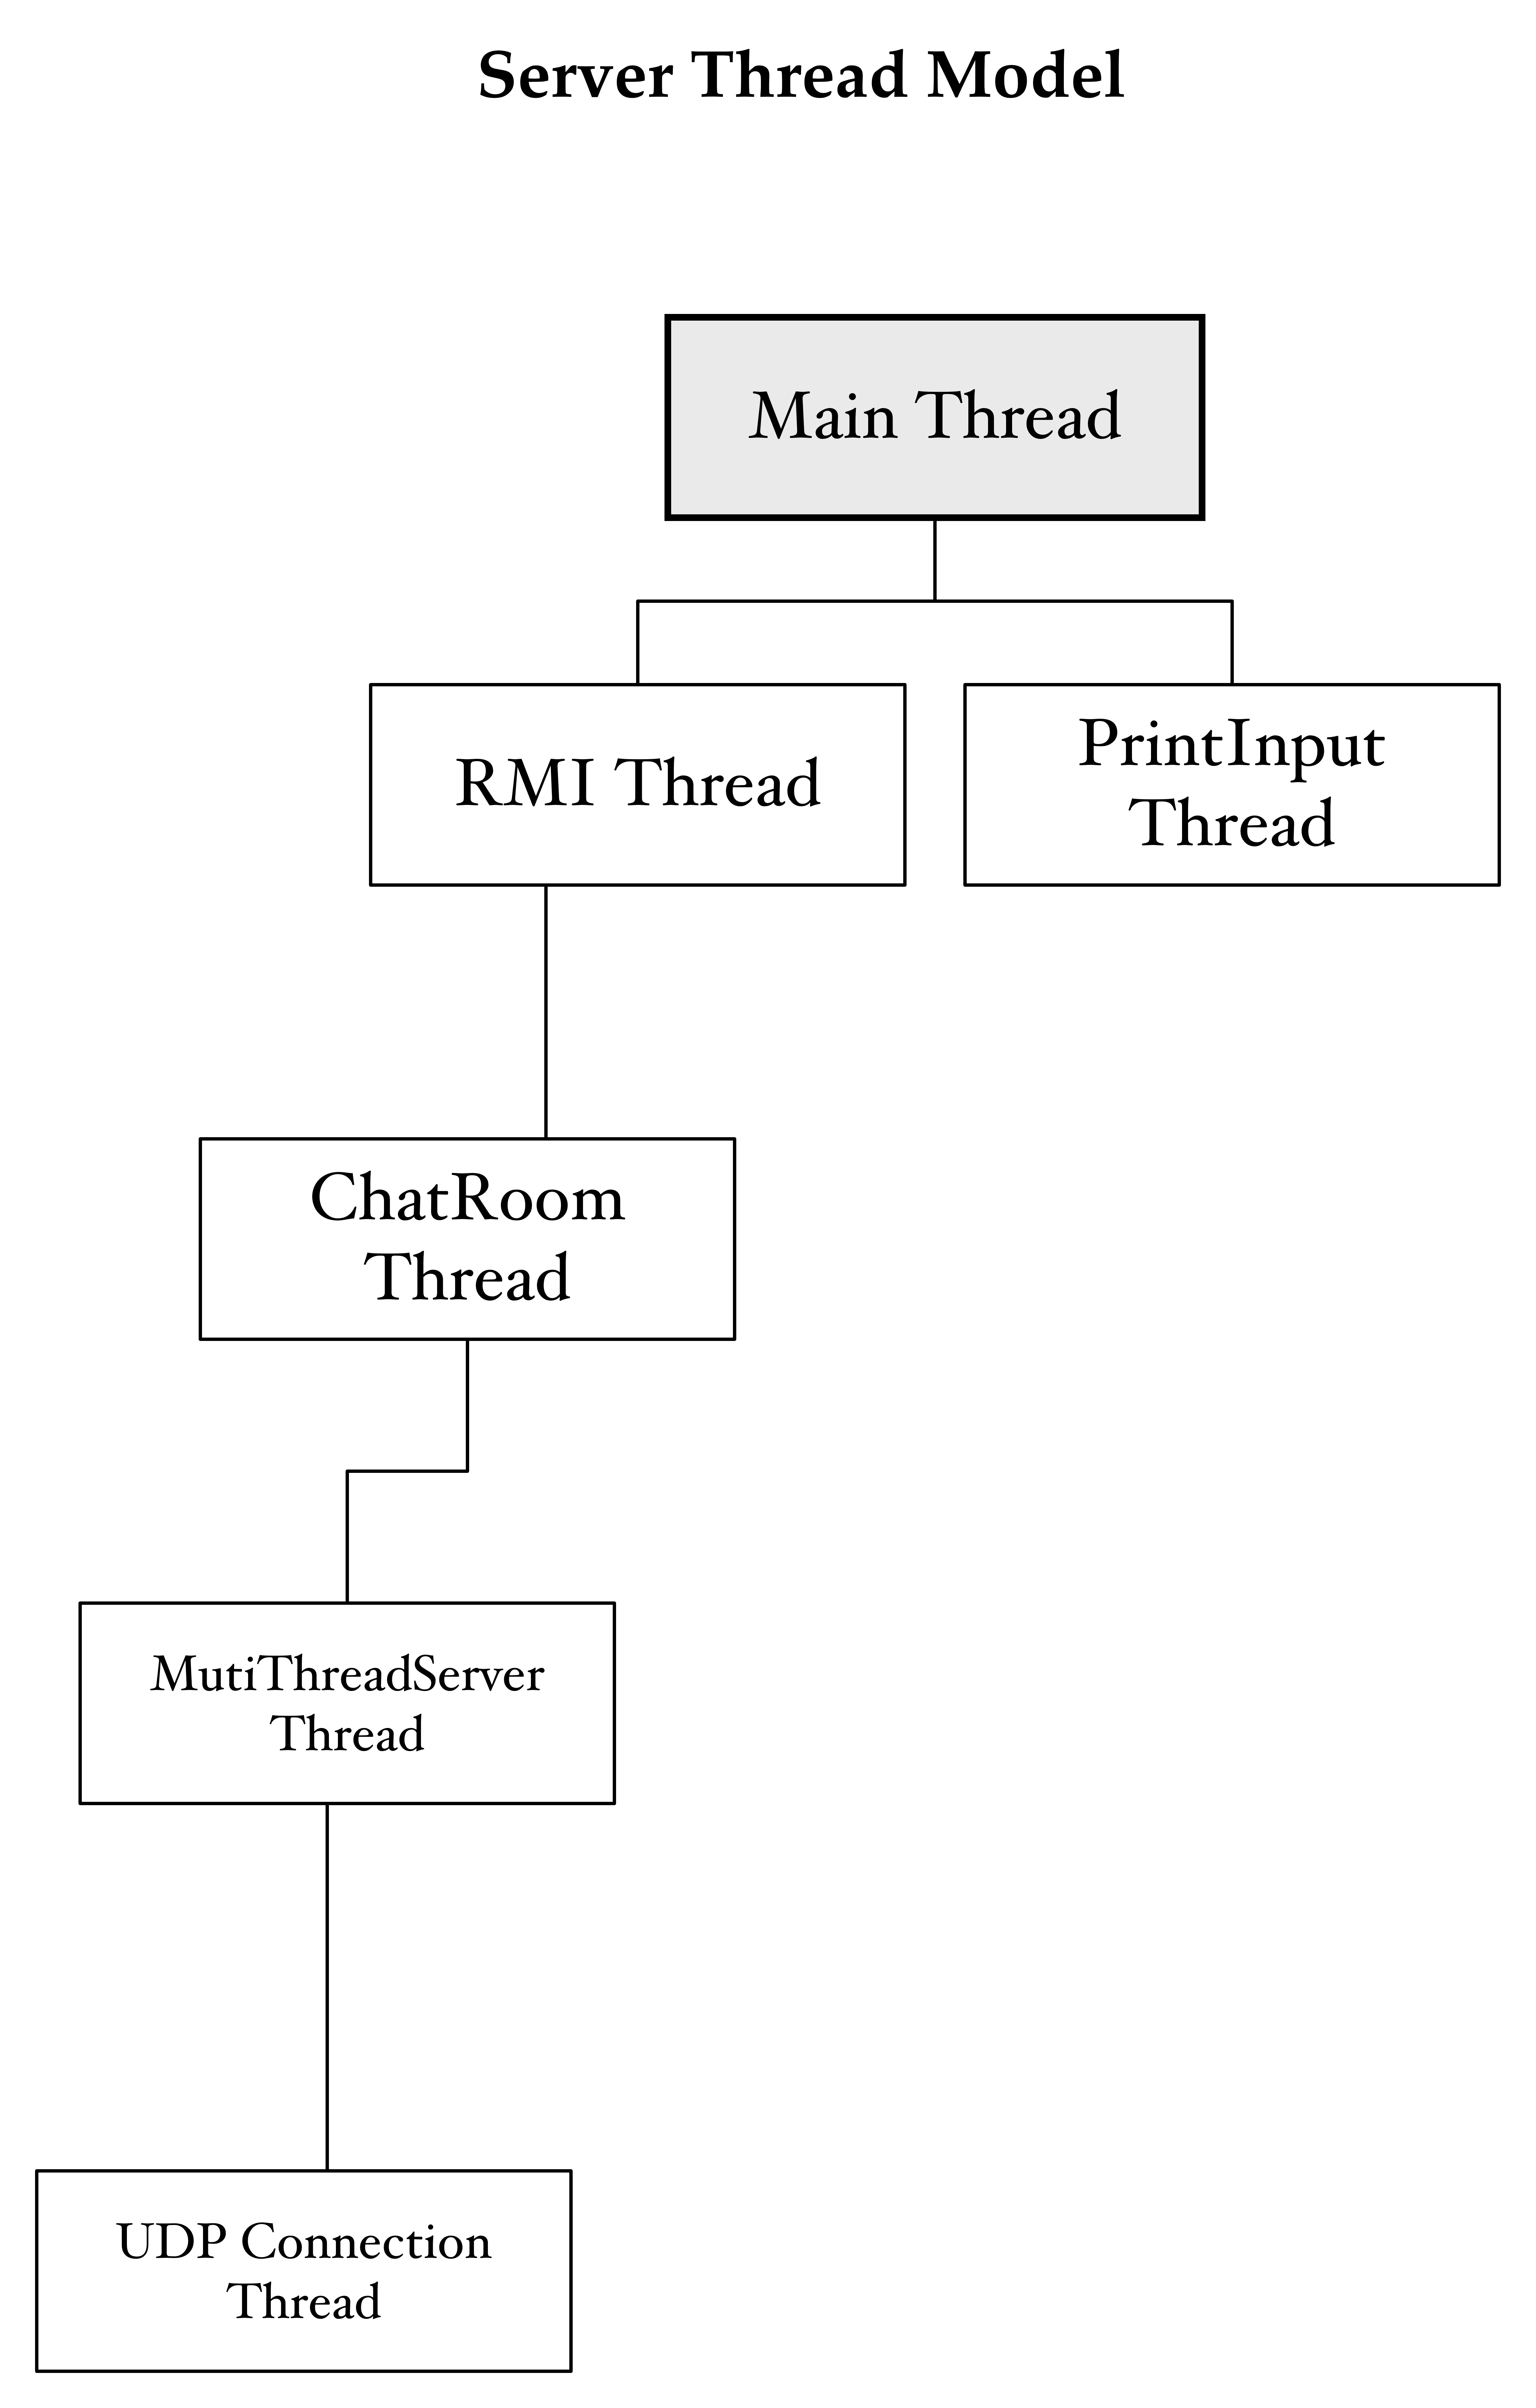
\includegraphics[scale=0.05]{Server}

\clearpage

The Client thread ask a username as a parameter at the first time and keep looping to promote user input their selection. The thread calls the RMI function implemented in server side to create chatroom. When the user choose to enter a chatroom, it starts a new thread and print out all message receiver from server. User can choose to enter different chat room, and quit chat room by entering "!q".\\

The PrintInput thread is created when the client choose to join a chat room. It prints a message to user's console and ack each message it received.\\

The ServerMain thread is a registry, it is used to register the RMI interface Message to RMI server and listen to the port 1099.\\
 accepts user's connection.The port of connection is randomly assigned by Server. Also, MutiThreadServer creates PrintOutput thread. In order to make entire system asynchronous, when a message send out,they PrintOutput thread block by variable "ack". In other word, Printout thread holds when it send a message but do not receive an ack message, whenever it receive the ack for current 
The Server thread extends the UnicastRemoteObject class and Message interface. it implements all methods in Message Interface. It creates a new thread of ChatRoom which when user choose to create a new chat room. The ChatRoom thread is assigned a port number. It contains two Hashmaps, the first one is used to  holds the chat room name and chat room instance, the second one is used to holds the chat room name and its port number.\\

The MutiThreadServer thread holds all threads of connection with users. whenever a user start a UDP connection, it is created by Server andmessage, it continues to output next string to client.\\

\section{Measurements}


\begin{table}[h]
\begin{tabular}{|l|l|l|l|}
\hline
ChatRoom Num/Registration and de-registration Num & 100   & 200  & 500  \\ \hline
100                                               & 0.387 & 0.57 & 0.85 \\ \hline
300                                               & 1.65  & 3.44 & 5.87 \\ \hline
500                                               & 2.49  & 3.47 & 6.23 \\ \hline
\end{tabular}
\caption{Latency are in second}
\label{my-label}
\end{table}

\begin{table}[h]
\begin{tabular}{|l|l|l|l|}
\hline
ChatRoom Num/Query Number & 100   & 200  & 500  \\ \hline
100                                               & 2.72 & 8.57 & 14.85 \\ \hline
300                                               & 5.25  & 12.54 & 21.27 \\ \hline
500                                               & 6.49  & 15.77 & 26.43 \\ \hline
\end{tabular}
\caption{Latency are in second}
\label{my-label}
\end{table}


\clearpage
From the above measurement result, we can conclude that, the number of chatroom has less effect on latency after it has established. In the first table, when increasing the number of registration and de-registration, the number slightly increase, because it implement in HashMap, it support random access in O(1). In table two, when we increase the query number, the latency increase largely due to the udp connection cost time to established and it cost O(500*500) time to transmit message.
\end{document}